\documentclass[aspectratio=169,11pt]{beamer}
\usepackage[T1]{fontenc}
\usepackage{booktabs}
\usepackage{amsmath}
\usepackage{tikz}
\usetikzlibrary{positioning}
\setbeamertemplate{navigation symbols}{}
\setbeamertemplate{footline}[frame number]
\setlength{\tabcolsep}{4pt}

\title{Knowledge distillation into a 17M encoder with 10\,\% of the labels}
\subtitle{Ettin-encoder-400m $\to$ Ettin-encoder-17m on SST-2}
\institute{Group project, Efficient Models course, ITMO 2026}
\date{}

\begin{document}

\begin{frame}
  \titlepage
\end{frame}

\begin{frame}{Motivation: labels are scarce, the accurate model is slow}
  \begin{columns}[T]
    \column{0.48\textwidth}
    \begin{itemize}
      \item Budget: gold labels for 10\,\% of the SST-2 train set (6,735 sentences); the other 60,614 sentences are available without labels
      \item With 10\,\% of SST-2 labels, the 400M teacher reaches 94.1\,\%, the 17M student only 84.3\,\%
      \item The student is 63 times faster on CPU
      \item Question: how much of the 100\,\%-label accuracy can the 17M student get from 10\,\% of the labels and a teacher?
    \end{itemize}
    \column{0.5\textwidth}
    \small
    \begin{tabular}{lrr}
      \toprule
      & Teacher & Student \\
      \midrule
      Parameters, M & 395.8 & 16.9 \\
      CPU, batch of 32, ms & 5,817 & 92 \\
      T4, sentences/s & 314 & 3,243 \\
      Accuracy, 10\,\% labels & 94.1 & 84.3 \\
      Accuracy, 100\,\% labels & 95.9 & 89.5 \\
      \bottomrule
    \end{tabular}

    \footnotesize SST-2 validation accuracy in \%, mean of 3 seeds (teacher at 100\,\%: 1), CPU: 2 threads
  \end{columns}
\end{frame}

\begin{frame}{Plan of work}
  \begin{enumerate}
    \item Fine-tune the teacher on a random 1, 5, 10, 25, 100\,\% of the SST-2 train set
    \item Train the student with cross-entropy (CE) on the same labels: the baseline
    \item Train the student with knowledge distillation (KD) on the labeled part only, and on all 67,349 sentences
    \item Replace the random 10\,\% by k-center selection
    \item Measure parameters, CPU latency, T4 throughput
    \item Vary the KD temperature and weight; repeat with 32M and 68M students; 3 teacher seeds at 10\,\%, a KD student from each
  \end{enumerate}
  \medskip
  Budget: 5 days, Kaggle T4 sessions of 12 hours; the 83 runs took 197 + 199 + 45 min in three sessions on one T4.
\end{frame}

\begin{frame}{Knowledge distillation (Hinton et al., 2015)}
  The student matches the teacher's class probabilities softened by temperature $T$:
  \[
    p_i = \frac{\exp(z_i / T)}{\sum_j \exp(z_j / T)}, \qquad
    \mathcal{L} = (1 - \alpha)\, \mathrm{CE}(y, p^{s}_{T=1}) + \alpha\, T^2\, \mathrm{KL}\bigl(p^{t}_{T} \,\|\, p^{s}_{T}\bigr)
  \]
  \begin{itemize}
    \item Soft targets carry how similar the classes are for each example; a one-hot label does not
    \item Gradients of the soft term scale as $1/T^2$, so it is multiplied by $T^2$
    \item MNIST: a small net made 146 test errors alone, 74 when trained on the soft targets of a large net (67 errors)
    \item Speech, 3\,\% of the training set: frame accuracy 44.5\,\% with hard targets, 57.0\,\% with soft targets, 58.9\,\% with all data
  \end{itemize}
  \footnotesize \url{https://arxiv.org/abs/1503.02531}
\end{frame}

\begin{frame}{Distillation through unlabeled task data}
  \begin{columns}[T]
    \column{0.5\textwidth}
    \textbf{Tang et al., 2019}: BERT $\to$ BiLSTM
    \begin{itemize}
      \item Transfer set: the train set plus sentences made by masking, part-of-speech-guided word replacement and n-gram sampling
      \item Mean squared error on logits, distillation term only ($\alpha = 0$ worked best)
      \item SST-2 test: BiLSTM 86.7 $\to$ 90.7\,\%; BERT-large 94.9\,\%
    \end{itemize}
    \footnotesize \url{https://arxiv.org/abs/1903.12136}
    \column{0.5\textwidth}
    \textbf{Turc et al., 2019}: Well-Read Students
    \begin{itemize}
      \item Pre-trained Distillation: masked language model pre-training of the compact model, then KD on unlabeled transfer data
      \item Pre-training the student matters even with millions of transfer examples
      \item 6-layer student, SST-2 test: 91.8\,\%
    \end{itemize}
    \footnotesize \url{https://arxiv.org/abs/1908.08962}
  \end{columns}
  \medskip
  Our \texttt{kdu} runs are Pre-trained Distillation with the SST-2 train sentences as the transfer set.
\end{frame}

\begin{frame}{Other distilled encoders}
  \begin{itemize}
    \item DistilBERT (Sanh et al., 2019): KD during pre-training; 40\,\% smaller than BERT-base, 60\,\% faster, 97\,\% of its GLUE score
    \item TinyBERT (Jiao et al., 2019): KD of embeddings, attention, hidden states and logits, general then task-specific, with data augmentation; 4 layers, 7.5 times smaller and 9.4 times faster than BERT-base, 96.8\,\% of its GLUE score
    \item Stanton et al., 2021: students often disagree with their teachers even when they could match them; the authors trace it mainly to optimization
  \end{itemize}
  \medskip
  We distill only logits: teacher and student have different widths and depths, and the loss stays one line.

  \medskip
  \footnotesize \url{https://arxiv.org/abs/1910.01108}, \url{https://arxiv.org/abs/1909.10351}, \url{https://arxiv.org/abs/2106.05945}
\end{frame}

\begin{frame}{Models: Ettin encoders}
  \begin{columns}[T]
    \column{0.56\textwidth}
    \begin{itemize}
      \item Ettin (Weller et al., 2025): paired encoders and decoders from 17M to 1B parameters, one recipe, one tokenizer, up to 2T tokens
      \item Architecture and recipe of ModernBERT (Warner et al., 2024): RoPE, alternating local and global attention, unpadding, 8,192-token context
      \item Teacher and student share the tokenizer: one tokenization for both, the teacher's logits are cached once
      \item 1B does not fit a T4 for AdamW fine-tuning, by estimate: 16 bytes per parameter, 16 GB, all of the T4's memory
    \end{itemize}
    \column{0.4\textwidth}
    \small
    \begin{tabular}{lr}
      \toprule
      Ettin encoder & Non-embedding, M \\
      \midrule
      400m, teacher & 344.3 \\
      68m & 42.6 \\
      32m & 12.7 \\
      17m, student & 4.0 \\
      \bottomrule
    \end{tabular}

    \footnotesize \url{https://arxiv.org/abs/2507.11412}, \url{https://arxiv.org/abs/2412.13663}
  \end{columns}
\end{frame}

\begin{frame}{Setup}
  \begin{columns}[T]
    \column{0.46\textwidth}
    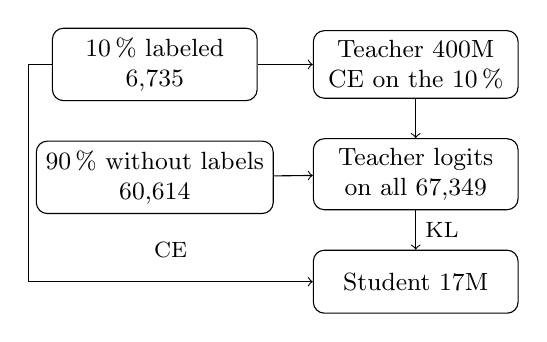
\begin{tikzpicture}[node distance=0.5cm and 0.6cm, every node/.style={draw, rounded corners, align=center, font=\small, minimum height=0.8cm, minimum width=2.6cm}]
      \node (lab) {10\,\% labeled\\6,735};
      \node (unl) [below=of lab] {90\,\% without labels\\60,614};
      \node (tea) [right=0.7cm of lab] {Teacher 400M\\CE on the 10\,\%};
      \node (log) [below=of tea] {Teacher logits\\on all 67,349};
      \node (stu) [below=of log] {Student 17M};
      \draw[->] (lab) -- (tea);
      \draw[->] (tea) -- (log);
      \draw[->] (unl) -- (log);
      \draw[->] (log) -- node[draw=none, minimum width=0pt, right, font=\footnotesize] {KL} (stu);
      \draw[->] (lab.west) -- ++(-0.3,0) |- node[draw=none, minimum width=0pt, pos=0.75, above, font=\footnotesize] {CE} (stu.west);
    \end{tikzpicture}
    \column{0.52\textwidth}
    \small
    \begin{tabular}{lll}
      \toprule
      Run & Student texts & Loss \\
      \midrule
      \texttt{hard\_p<p>} & p\,\% labeled & CE \\
      \texttt{kd\_p<p>} & p\,\% labeled & CE + KL \\
      \texttt{kdu\_p<p>} & all 67,349 & CE + KL \\
      \bottomrule
    \end{tabular}

    \medskip
    \begin{itemize}
      \item \texttt{kdu}: CE on the labeled sentences, KL on all
      \item GLUE SST-2; the validation split (872) is the test set, no dev set, last step evaluated
      \item $T = 2$, $\alpha = 0.5$; AdamW, batch 32, fp16; teacher LR 3e-5, 3 epochs; student LR 1e-4, 5 epochs
      \item Students: 3 seeds, from the seed-0 teacher; teachers: 1 seed, \texttt{teacher\_p10}: 3
    \end{itemize}
  \end{columns}
\end{frame}

\begin{frame}{Frameworks and reproducibility}
  \begin{itemize}
    \item PyTorch 2.11, Hugging Face Transformers 5.16 and Datasets; matplotlib for the figures
    \item uv with a lock file and a Dockerfile for local runs; Kaggle notebook for the T4
    \item Two scripts: \texttt{kd.py} (data, training, KD loss, k-center, benchmark, list of runs), \texttt{plots.py} (tables, figure)
    \item Each run writes \texttt{results/runs/<run>.json} with metrics and environment; a run whose file exists is skipped, so a new Kaggle session resumes from the output of the previous one
    \item Teacher logits and k-center indices are cached in \texttt{results/}
    \item \texttt{kd.py --smoke}: the whole pipeline on CPU, 13 min in the Docker image on a Mac
  \end{itemize}
\end{frame}

\begin{frame}{KD on unlabeled sentences closes 72\,\% of the gap at 10\,\% labels}
  \begin{columns}[T]
    \column{0.45\textwidth}
    \small
    \begin{tabular}{lr}
      \toprule
      Run & Accuracy, \% \\
      \midrule
      \texttt{teacher\_p10} & 94.1 $\pm$ 0.7 \\
      \texttt{hard\_p10} & 84.3 $\pm$ 1.3 \\
      \texttt{kd\_p10} & 84.1 $\pm$ 0.6 \\
      \texttt{kdu\_p10} & 88.1 $\pm$ 0.2 \\
      \texttt{hard\_p100} & 89.5 $\pm$ 0.6 \\
      \texttt{kd\_p100} & 89.0 $\pm$ 0.3 \\
      \bottomrule
    \end{tabular}

    \footnotesize Mean $\pm$ std over 3 seeds
    \column{0.52\textwidth}
    \begin{itemize}
      \item \texttt{kdu\_p10} gained 3.8 points over \texttt{hard\_p10}, 72\,\% of the 5.2-point gap to \texttt{hard\_p100}
      \item The gain came from the 90\,\% without labels: KD on the labeled 10\,\% alone was within the seed spread of CE
      \item With all labels, KD from a 95.9\,\% teacher did not raise the student
      \item Teacher seeds: 93.7, 94.8, 93.7\,\%; KD students from them: 88.1, 88.6, 88.4\,\%
    \end{itemize}
  \end{columns}
\end{frame}

\begin{frame}{KL only with 10\,\% of the labels matched CE with all labels}
  \begin{columns}[T]
    \column{0.45\textwidth}
    \small
    \begin{tabular}{lrrr}
      \toprule
      Run & $T$ & $\alpha$ & Accuracy, \% \\
      \midrule
      \texttt{kdu\_p10\_t1} & 1 & 0.5 & 87.4 $\pm$ 0.3 \\
      \texttt{kdu\_p10} & 2 & 0.5 & 88.1 $\pm$ 0.2 \\
      \texttt{kdu\_p10\_t4} & 4 & 0.5 & 88.8 $\pm$ 0.2 \\
      \texttt{kdu\_p10\_a1} & 2 & 1 & 89.7 $\pm$ 0.3 \\
      \texttt{kdu\_p10\_t4a1} & 4 & 1 & 89.3 $\pm$ 0.3 \\
      \texttt{hard\_p100} & & 0 & 89.5 $\pm$ 0.6 \\
      \bottomrule
    \end{tabular}

    \footnotesize 17M student, 10\,\% labels except \texttt{hard\_p100}, 3 seeds
    \column{0.52\textwidth}
    \begin{itemize}
      \item KL only ($\alpha = 1$): +1.6 points over $\alpha = 0.5$, within the seed spread of CE on all 67,349 labels
      \item The student saw the gold labels only through a teacher trained on 10\,\% of them
      \item Each step of $T$ from 1 to 2 to 4 added 0.7 points
      \item Tang et al.\ also found the distillation term alone best
      \item With $\alpha = 1$, $T = 4$ did not help: $-0.4$, within the spread
    \end{itemize}
  \end{columns}
\end{frame}

\begin{frame}{With KD, 5\,\% of the labels beat 25\,\% without it}
  \begin{columns}[T]
    \column{0.55\textwidth}
    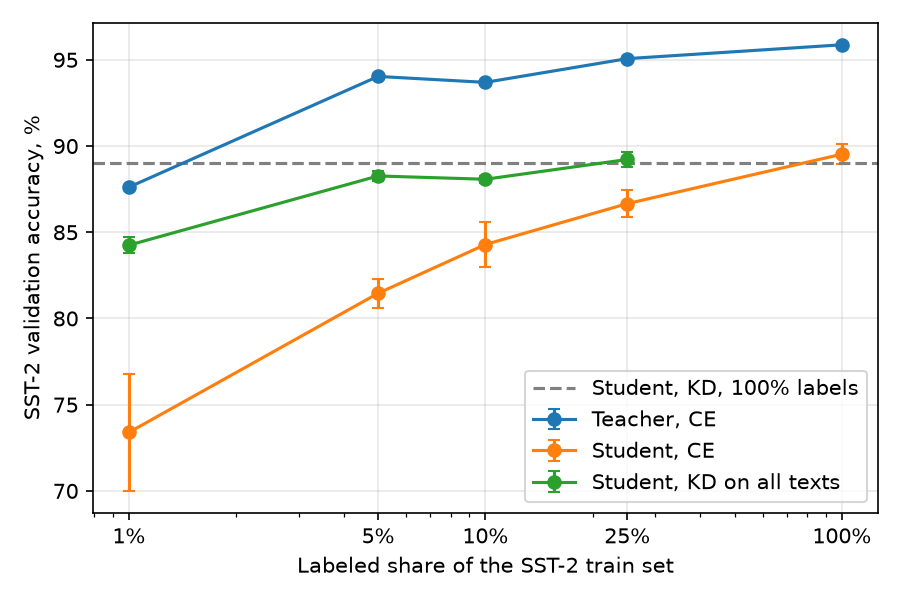
\includegraphics[width=\textwidth]{../results/figures/label_curve.png}
    \column{0.43\textwidth}
    \small
    \begin{tabular}{rrr}
      \toprule
      Labels & \texttt{hard}, \% & \texttt{kdu}, \% \\
      \midrule
      1\,\% & 73.4 $\pm$ 3.4 & 84.3 $\pm$ 0.5 \\
      5\,\% & 81.5 $\pm$ 0.8 & 88.3 $\pm$ 0.3 \\
      10\,\% & 84.3 $\pm$ 1.3 & 88.1 $\pm$ 0.2 \\
      25\,\% & 86.7 $\pm$ 0.8 & 89.2 $\pm$ 0.4 \\
      100\,\% & 89.5 $\pm$ 0.6 & \\
      \bottomrule
    \end{tabular}

    \medskip
    \begin{itemize}
      \item KD with 1\,\% matched CE with 10\,\%
      \item The gain shrank from 10.9 points at 1\,\% to 2.6 at 25\,\%
      \item KD seed spread: 0.2--0.5, CE: 0.6--3.4
    \end{itemize}
  \end{columns}
\end{frame}

\begin{frame}{A larger student gains less from KD}
  \begin{columns}[T]
    \column{0.55\textwidth}
    \small
    \begin{tabular}{lrrr}
      \toprule
      Student & \texttt{hard\_p10} & \texttt{kdu\_p10} & \texttt{hard\_p100} \\
      \midrule
      Ettin 17M & 84.3 $\pm$ 1.3 & 88.1 $\pm$ 0.2 & 89.5 $\pm$ 0.6 \\
      Ettin 32M & 88.0 $\pm$ 1.0 & 90.2 $\pm$ 0.5 & 89.6 $\pm$ 0.9 \\
      Ettin 68M & 89.6 $\pm$ 0.4 & 91.1 $\pm$ 0.4 & 92.4 $\pm$ 0.7 \\
      \bottomrule
    \end{tabular}

    \footnotesize Accuracy in \%, 3 seeds, $T = 2$, $\alpha = 0.5$, the same LR and epochs for all sizes
    \column{0.42\textwidth}
    \begin{itemize}
      \item KD gain at 10\,\% labels: 3.8, 2.2, 1.5 points
      \item CE with 10\,\% labels rose from 84.3 to 89.6\,\%
      \item 32M: KD with 10\,\% within the seed spread of CE with all labels
      \item 68M: KD closed 54\,\% of the gap
      \item CE with all labels: 17M and 32M both at 89.5--89.6\,\%
    \end{itemize}
  \end{columns}
\end{frame}

\begin{frame}{K-center selection of the 10\,\% lowered accuracy}
  \begin{columns}[T]
    \column{0.48\textwidth}
    \begin{itemize}
      \item K-center greedy (Sener \& Savarese, 2018): pick the point farthest from the chosen set until 10\,\%; a 2-approximation of the k-center problem
      \item Space: mean-pooled embeddings of the pretrained 400M teacher
      \item Two 2025 projects found selections with k-center or k-means better than random for CE on SST-2
    \end{itemize}
    \footnotesize \url{https://arxiv.org/abs/1708.00489}
    \column{0.5\textwidth}
    \small
    \begin{tabular}{lrr}
      \toprule
      Run & Random, \% & K-center, \% \\
      \midrule
      \texttt{teacher}, seed 0 & 93.7 & 92.8 \\
      \texttt{hard} & 84.3 $\pm$ 1.3 & 79.1 $\pm$ 1.0 \\
      \texttt{kdu} & 88.1 $\pm$ 0.2 & 86.7 $\pm$ 0.3 \\
      \bottomrule
    \end{tabular}

    \medskip
    \begin{itemize}
      \item CE lost 5.2 points, KD 1.4
      \item Positive share: 57.3\,\% in the k-center subset, 55.2\,\% in the random one
    \end{itemize}
  \end{columns}
\end{frame}

\begin{frame}{Previous projects on SST-2 with 10\,\% of the labels}
  \footnotesize
  \begin{tabular}{llrrl}
    \toprule
    Project (ITMO 2025) & Model & 100\,\% & Random 10\,\% & Best 10\,\% \\
    \midrule
    ITMO-EDLM/data-efficiency & ModernBERT-base & 94.7 & 75.8 & 92.1, entropy + k-center \\
    llm-data-selection-bert & bert-tiny, 4.4M & 81.9 & 74.7 & 79.2, quality + diversity \\
    train-data-sampling & ModernBERT-base & 95.1 & 92.1 & 92.9, k-means \\
    This project, student & Ettin 17M & 89.5 & 84.3 & 88.1, KD on all texts \\
    \bottomrule
  \end{tabular}

  \medskip
  \normalsize
  \begin{itemize}
    \item All three selected data and trained with CE; none used a teacher
    \item One run per config in each; the same ModernBERT-base with random 10\,\% got 75.8 and 92.1
  \end{itemize}
\end{frame}

\begin{frame}{The student is 63 times faster than the teacher on CPU}
  \begin{columns}[T]
    \column{0.58\textwidth}
    \footnotesize
    \begin{tabular}{lrrr}
      \toprule
      Model & Params, M & CPU, ms & T4, sent/s \\
      \midrule
      Ettin-encoder-400m & 395.8 & 5,817 & 314 \\
      Ettin-encoder-68m & 68.4 & 736 & 1,278 \\
      Ettin-encoder-32m & 32.0 & 237 & 2,423 \\
      Ettin-encoder-17m & 16.9 & 92 & 3,243 \\
      \bottomrule
    \end{tabular}

    \footnotesize CPU: median of 10 forward passes over 32 test sentences, 2 PyTorch threads, Kaggle; T4: fp16 over the 872 test sentences
    \column{0.38\textwidth}
    \begin{itemize}
      \item 23 times fewer parameters, 86 times fewer outside the embedding matrix
      \item 10.3 times the T4 throughput
      \item 68M is 8 times slower than 17M on CPU
      \item KD cost: one teacher pass over 67,349 sentences, cached
    \end{itemize}
  \end{columns}
\end{frame}

\begin{frame}{Conclusions and next steps}
  \begin{itemize}
    \item With 10\,\% of SST-2 labels, KD through all train sentences gave the 17M student 89.7\,\% (KL only), against 84.3\,\% with CE and 89.5\,\% with all labels
    \item The gain came from the sentences without labels: KD on the labeled 10\,\% alone matched CE
    \item KD with 5\,\% of the labels beat CE with 25\,\%; KD runs varied less between seeds
    \item The KD gain shrank with student size, from 3.8 points at 17M to 1.5 at 68M
    \item K-center selection hurt both CE and KD students
  \end{itemize}
  \medskip
  Next steps:
  \begin{itemize}
    \item KL only ($\alpha = 1$) at every label share and student size
    \item Tune the student's LR and epochs on a dev split carved from the labeled 10\,\%
    \item Augmented or out-of-domain transfer sets
  \end{itemize}
  \medskip
  \footnotesize \url{github.com/PE51K/itmo-ai-talent-hub-efficient-models-course/tree/main/project}
\end{frame}

\end{document}
